\section{Pointwise smoothing thresholds}
\label{sec:thresholds}

The safe regime uses \(\rho\) uniformly over all centers and multipliers, but
a fixed KKT pair may require less curvature.  This section gives the exact
pointwise threshold and separates the value-defined condition from attainment
or local solution of the inner problem.

\subsection{Support curvature and the exact pointwise threshold}

The global constant \(\rho\) controls every center and every multiplier, but a
fixed slope at a fixed point may admit a sharper global quadratic support.
Motivated by the level-proximal subdifferential in
\cref{eq:level-prox}, define the extended-valued
\emph{support curvature}
\begin{equation}
  \kappa_f(x\mid g)
  :=
  \inf\left\{
    \beta\ge0:
    g\in\partial_{\mathrm p}^{\beta}f(x)
  \right\},
  \qquad \inf\varnothing:=+\infty.
  \label{eq:support-curvature}
\end{equation}

\begin{lemma}[Quotient representation of support curvature]
  \label{lem:support-curvature}
  For \(x\in\operatorname{dom}f\) and \(g\in\R^n\),
  \begin{equation}
    \kappa_f(x\mid g)
    =
    \sup_{\substack{u\in\operatorname{dom}f\\u\ne x}}
    \frac{
      2[f(x)-f(u)+\ip{g}{u-x}]_+
    }{\norm{u-x}^2}.
    \label{eq:support-curvature-quotient}
  \end{equation}
  The supremum of an empty set is understood as zero.  Moreover, for every
  finite \(\beta\ge0\),
  \begin{equation}
    g\in\partial_{\mathrm p}^{\beta}f(x)
    \quad\Longleftrightarrow\quad
    \beta\ge\kappa_f(x\mid g).
    \label{eq:support-curvature-membership}
  \end{equation}
\end{lemma}

\begin{proof}
  By \cref{eq:level-prox}, membership
  \(g\in\partial_{\mathrm p}^{\beta}f(x)\) is equivalent, for every
  \(u\in\operatorname{dom}f\setminus\{x\}\), to
  \[
    \beta
    \ge
    \frac{2[f(x)-f(u)+\ip{g}{u-x}]}{\norm{u-x}^2}.
  \]
  Since \(\beta\ge0\), the right-hand side can be replaced by its positive
  part.  Taking the supremum over
  \(u\in\operatorname{dom}f\setminus\{x\}\) proves
  \cref{eq:support-curvature-quotient}; the same family of closed
  inequalities proves \cref{eq:support-curvature-membership}, including
  attainment at a finite threshold.
\end{proof}

We apply this support calculation to the stationary candidates identified
by the safe SDG.  At a KKT pair, feasibility holds and stationarity selects
the slope \(g=-A^\top y\in\partial f(x)\).  The question is how far the
primal smoothing can be reduced while this pair remains a zero of the gap.
For this purpose, define the Lagrangian support threshold, for any
\((x,y)\in\operatorname{dom}f\times\R^m\), by
\begin{equation}
  \begin{split}
  \beta_{\crit}(x,y)
  &:=
  \kappa_f(x\mid-A^\top y)\\
  &=
  \sup_{\substack{u\in\operatorname{dom}f\\u\ne x}}
  \frac{2[\Lagr(x,y)-\Lagr(u,y)]_+}{\norm{u-x}^2}.
  \end{split}
  \label{eq:beta-crit}
\end{equation}
Thus \(\beta_{\crit}(x,y)\) is precisely the least curvature for which the
relevant Lagrangian slope belongs to the level-proximal subdifferential.  It
is a global property at the \emph{fixed} multiplier \(y\).  A distinct,
multiplier-free curvature localized to a feasible ball is introduced in
\cref{eq:local-support-threshold} when proximal escape is developed.

The same number admits two equivalent optimization interpretations.  For
every \(\beta>0\),
\begin{equation}
  \begin{split}
  \beta\ge\beta_{\crit}(x,y)
  &\quad\Longleftrightarrow\quad
  x\in\argmin_u
  \left\{
    \Lagr(u,y)+\frac{\beta}{2}\norm{u-x}^{2}
  \right\}\\
  &\quad\Longleftrightarrow\quad
  x\in
  P_{\beta^{-1}}
  \left(x-\beta^{-1}A^\top y\right).
  \end{split}
  \label{eq:beta-crit-equivalent-models}
\end{equation}
The first equivalence is the global support inequality with all terms moved
to one side; the second follows by completing the square as in
\cref{eq:lagrangian-completing-square-expanded}.  Consequently
\begin{equation}
  \beta_{\crit}(x,y)
  =
  \inf\left\{
    \beta\ge0:
    x\in\argmin_u
      \left(\Lagr(u,y)+\frac{\beta}{2}\norm{u-x}^{2}\right)
  \right\}.
  \label{eq:beta-crit-model-infimum}
\end{equation}
The support inequality is closed in \(\beta\), and the curvature monotonicity
in \cref{eq:level-prox-monotonicity} makes the admissible curvatures upward
closed.  Hence, when the infimum is finite, it is attained and the
support/model curvatures form the closed ray
\([\beta_{\crit}(x,y),+\infty)\), rather than merely an open sufficient
range.  For a feasible pair \(Ax=b\), the positive curvatures producing
zero SDG are exactly those satisfying \(\beta_x\ge\beta_{\crit}(x,y)\).
For \(Ax\ne b\), no positive curvature produces zero SDG.

\begin{theorem}[Pointwise zero-gap criterion]
  \label{thm:pointwise-threshold}
  Let \(f\) be proper and lower semicontinuous.  Fix
  \((x,y)\in\operatorname{dom}f\times\R^m\) and
  \(\beta_x,\beta_y>0\).  Interpret the SDG through its global infimum.  Then
  \begin{equation}
    \G_{\beta_x,\beta_y}(x,y)=0
    \quad\Longleftrightarrow\quad
    Ax=b\ \text{ and }\ \beta_x\ge\beta_{\crit}(x,y).
    \label{eq:threshold-equivalence}
  \end{equation}
  Every zero in \cref{eq:threshold-equivalence} is a KKT pair.  If, in
  addition, \(f\) is \(\rho\)-weakly convex and \((x,y)\) is KKT, then
  \begin{equation}
    0\le\beta_{\crit}(x,y)\le\rho.
    \label{eq:threshold-rho-bound}
  \end{equation}
\end{theorem}

\begin{proof}
  By \Cref{thm:arbitrary-beta}, zero gap is equivalent to feasibility and
  \(-A^\top y\in\partial_{\mathrm p}^{\beta_x}f(x)\).  Applying
  \cref{eq:support-curvature-membership} and
  \(\beta_{\crit}(x,y)=\kappa_f(x\mid-A^\top y)\) proves
  \cref{eq:threshold-equivalence}.  The KKT implication is already part of
  \Cref{thm:arbitrary-beta}.  At a KKT pair,
  \(-A^\top y\in\partial f(x)\); weak convexity and
  \cref{eq:level-prox-weak-convex} then give
  \(-A^\top y\in\partial_{\mathrm p}^{\rho}f(x)\).  Therefore
  \(\kappa_f(x\mid-A^\top y)\le\rho\), proving
  \cref{eq:threshold-rho-bound}.
\end{proof}

For \(\rho>0\), the distinction at the boundary \(\beta_x=\rho\) is exact.  At a KKT pair,
\cref{eq:threshold-rho-bound} and
\cref{eq:threshold-equivalence} show that the SDG vanishes for every
\(\beta_x\ge\rho\), including equality.  Thus the strict inequality in
\Cref{thm:safe-zero-set} is not needed for the value-defined zero-set
equivalence.  It is needed for a \emph{uniform computational statement}:
when \(\beta_x>\rho\), every inner model is strongly convex, coercive, and
has a unique minimizer; when \(\beta_x=\rho\), the inner model is only
convex, and its behavior away from a zero can vary.

For example, let \(\rho>0\) and
\(f(u)=-\rho\norm{u}^{2}/2\) with no effective constraint.  At the boundary,
\begin{equation}
  f(u)+\frac{\rho}{2}\norm{u-x}^{2}
  =
  -\rho\ip{x}{u}+\frac{\rho}{2}\norm{x}^{2}.
  \label{eq:boundary-flat-linear-model}
\end{equation}
If \(x\ne0\), the inner infimum is \(-\infty\); at the stationary point
\(x=0\), the model is constant and every \(u\) is a minimizer.  In contrast,
the quartic model in \cref{ex:double-well} has the unique boundary minimizer
\(u=0\).  The boundary can therefore be attained uniquely, attained
nonuniquely, or fail to have a finite value, depending on the center and the
recession behavior.  What is lost at equality is the uniform
strong-convexity guarantee, not the KKT-to-zero implication at a KKT pair.

\begin{corollary}[Global saddle case]
  Let \(x\in\Cset\cap\operatorname{dom}f\) and \(y\in\R^m\).  Then
  \(\beta_{\crit}(x,y)=0\) if and only if
  \(x\in\argmin_u\Lagr(u,y)\).  Equivalently, \((x,y)\) is a global saddle
  pair of the ordinary Lagrangian.
\end{corollary}

Thus the spectrum between \(0\) and \(\rho\) has a precise interpretation.
A global saddle needs no primal smoothing.  If
\(x\notin\argmin_u\Lagr(u,y)\), then
\(\beta_{\crit}(x,y)>0\); here globality refers to minimization of the
all-space Lagrangian at the fixed multiplier \(y\), not to minimization of
\(f\) over \(\Cset\).  The uniform constant \(\rho\) is only a worst-case
upper bound, and exact evaluation of the pointwise threshold is a global
supremum over \(u\).

\subsection{Sharp examples and inner-solve requirements}

Existence of a global proximal minimizer is distinct from convexity of the
inner model.  A proper lower-semicontinuous function is
\emph{prox-bounded} if its Moreau envelope is finite at some center for some
positive parameter.  Its threshold is
\begin{equation}
  \lambda_f^{\mathrm{pb}}
  :=
  \sup\left\{
    \lambda>0:
    \Moreau_\lambda(z)>-\infty
    \ \text{for some }z\in\R^n
  \right\}.
  \label{eq:prox-boundedness-threshold}
\end{equation}
For a proper lower-semicontinuous prox-bounded function, the standard
proximal-attainment theorem states that, for every
\(0<\lambda<\lambda_f^{\mathrm{pb}}\), the proximal set \(P_\lambda(z)\)
is nonempty and compact and the envelope is finite at every center
\citep[Definition~1.23 and Theorem~1.25]{RockafellarWets1998}.  The theorem
therefore guarantees finiteness, attainment, and compactness; uniqueness and
convexity require additional structure.

Completing the square in the SDG inner model shows that this result applies
with \(\lambda=\beta_x^{-1}\) and center
\(x-\beta_x^{-1}A^\top y\).  Thus
\begin{equation}
  \beta_x>\left(\lambda_f^{\mathrm{pb}}\right)^{-1}
  \quad\Longrightarrow\quad
  m_{\beta_x}(x,y)\ \text{is finite and attained},
  \label{eq:prox-boundedness-attainment}
\end{equation}
where \(1/(+\infty)=0\).  If \(f\) is \(\rho\)-weakly convex, its global
quadratic minorant implies
\(\lambda_f^{\mathrm{pb}}\ge1/\rho\), with the usual convention for
\(\rho=0\).  Hence \(\beta_x>\rho\) lies strictly inside the general
attainment range, but is stronger because it also guarantees a unique
strongly convex inner problem.

At the threshold
\(\lambda=\lambda_f^{\mathrm{pb}}\), attainment must be checked separately.
All quartic objectives below are bounded from below, so
\(\lambda_f^{\mathrm{pb}}=+\infty\): their inner minima are attained for
every \(\beta_x>0\).  Consequently, the false-zero phenomenon below arises
from selection of a nonglobal local branch despite global attainment.

\subsubsection{Sharp quartic threshold examples}

\begin{example}[Double well with a unique feasible point]
  \label{ex:double-well}
  Consider the equality-constrained problem
  \[
    \min_{t\in\R}\left\{
      f(t):=\frac14t^4-\frac12t^2
    \right\}
    \qquad\text{subject to}\qquad t=0.
  \]
  The objective is \(1\)-weakly convex.  The unique feasible point \(x=0\),
  with \(y=0\), is therefore globally optimal for the constrained problem and
  is a KKT pair.  Yet its primal proximal model is
  \[
    \frac14u^4+\frac{\beta_x-1}{2}u^2.
  \]
  Direct minimization gives
  \begin{equation}
    \G_{\beta_x,\beta_y}(0,0)
    =\frac14(1-\beta_x)_+^2.
    \label{eq:double-well-gap}
  \end{equation}
  Indeed, with \(a=1-\beta_x\), the proximal model is
  \(\varphi(u)=u^4/4-au^2/2\).  If \(a>0\), its global minimizers are
  \(u=\pm\sqrt a\), with value \(-a^2/4\); if \(a\le0\), the center \(u=0\)
  is globally minimizing.  Subtracting the global model value from the
  center value proves \cref{eq:double-well-gap}.
  Hence the SDG is positive for every \(0<\beta_x<1\) and vanishes for
  \(\beta_x\ge1\).  The pair is globally optimal \emph{under the constraint},
  but the SDG inner model compares it with infeasible points and sees the two
  wells.  This disproves a parameter-free global-optimality interpretation.
\end{example}

Here \(\beta_{\crit}(0,0)=1=\rho\), and at the boundary the proximal model is
\(u^4/4\) with a unique minimizer.  This is the unique-attainment branch of
the boundary alternatives described by
\cref{eq:boundary-flat-linear-model}.  The example also separates two notions
of globality: \(x=0\) is the unique global minimizer on the feasible set
\(\{0\}\), but it is not a global minimizer of the all-space Lagrangian.
Accordingly its pointwise Lagrangian support threshold is positive.

Consider the tilted quartic
\begin{equation}
  h(t)=\frac14t^4-\frac12t^2+0.1t.
  \label{eq:tilted-quartic}
\end{equation}
It is \(1\)-weakly convex and has three stationary points.  Their thresholds
can be obtained without a numerical global optimizer.  If \(x\) is any root
of \(h'(x)=x^3-x+0.1=0\) and \(u=x+d\), exact expansion gives
\begin{equation}
  h(x+d)-h(x)+\frac{\beta}{2}d^2
  =
  \frac{d^2}{4}
  \left[
    d^2+4xd+2(3x^2-1+\beta)
  \right].
  \label{eq:tilted-quartic-factorization}
\end{equation}
The quadratic bracket has its minimum at \(d=-2x\), where its value is
\(2(x^2-1+\beta)\).  Hence
\begin{equation}
  \beta_{\crit}(x,0)=(1-x^2)_+ .
  \label{eq:tilted-quartic-exact-threshold}
\end{equation}
This exact formula gives \cref{tab:tilted-thresholds}.  The global minimizer
has threshold zero, the local maximum almost reaches the uniform bound, and
the higher-valued local minimum needs only about one tenth of that bound.

\begin{center}
  \captionsetup{hypcap=false}
  \centering
  \captionof{table}{Stationary points and exact thresholds for the tilted
  quartic in \eqref{eq:tilted-quartic}.  Numerical values are rounded.}
  \label{tab:tilted-thresholds}
  \begin{tabular}{lS[table-format=-1.10]S[table-format=-1.10]S[table-format=1.9]}
    \toprule
    Type & {$x$} & {$h(x)$} & {$\beta_{\crit}$}\\
    \midrule
    Global minimum       & -1.0466805318 & -0.3523860738 & 0\\
    Local maximum        &  0.1010312579 &  0.0050255156 & 0.989792685\\
    Higher-valued local minimum &  0.9456492739 & -0.1526394418 & 0.105747451\\
    \bottomrule
  \end{tabular}
\end{center}

A two-dimensional example shows the multiplier's role in the Lagrangian
support calculation:
\[
  f(x_1,x_2)=\sum_{i=1}^2
       \left(\frac14x_i^4-\frac12x_i^2\right),
  \qquad x_1+x_2=1.
\]
The KKT equations reduce to
\[
  x_1^3-x_1+y=0,\qquad
  x_2^3-x_2+y=0,\qquad
  x_1+x_2=1,
\]
and give the three pairs
\[
  (x_1,x_2,y)
  =
  (0,1,0),\quad(1,0,0),\quad
  \left(\frac12,\frac12,\frac38\right).
\]
Before comparing their support thresholds, consider the feasible geometry.
Parametrizing the line by \(x=(t,1-t)\) gives
\[
  f(t,1-t)=\frac12t^2(t-1)^2-\frac14.
\]
Thus \((0,1)\) and \((1,0)\) are global constrained minimizers, whereas
\((1/2,1/2)\) is a strict local maximum on the line.  The support calculation
below instead compares all-space Lagrangian values at each fixed multiplier.

At an endpoint pair, the coordinate centered at zero has model difference
\begin{equation}
  \frac14d^4+\frac{\beta-1}{2}d^2,
  \label{eq:endpoint-coordinate-model}
\end{equation}
which is nonnegative for every \(d\) exactly when \(\beta\ge1\); the
coordinate centered at one already globally minimizes its unregularized
summand.  Thus the endpoint pairs have
\(\beta_{\crit}=1\).

At the symmetric pair, separability reduces the calculation to one
coordinate.  With \(u_i=\frac12+d_i\), stationarity cancels the linear term
and
\begin{equation}
  \begin{split}
  &\left(\frac14u_i^4-\frac12u_i^2+\frac38u_i\right)
  -\left(\frac14\left(\frac12\right)^4
         -\frac12\left(\frac12\right)^2
         +\frac38\left(\frac12\right)\right)
  +\frac{\beta}{2}d_i^2\\
  &\qquad =
  \frac{d_i^2}{4}
  \left[(d_i+1)^2+2\beta-\frac32\right].
  \end{split}
  \label{eq:symmetric-coordinate-factorization}
\end{equation}
This expression is nonnegative for every \(d_i\) if and only if
\(\beta\ge3/4\).  Therefore
\(\beta_{\crit}(\frac12,\frac12,\frac38)=3/4\).  At the critical value,
\(d_i=0\) and \(d_i=-1\) are both global minimizers of the scalar inner
model, so the SDG is already zero below the uniform weak-convexity curvature
\(\rho=1\), although the proximal map is set-valued.  The multiplier \(3/8\)
is essential in this calculation because \cref{eq:beta-crit} uses the
all-space Lagrangian and therefore includes infeasible comparison points.

The constrained maximum therefore has the smaller Lagrangian support
threshold.  As \Cref{fig:affine-quartic-geometry} illustrates, the order of
these thresholds does not rank the points by constrained optimality.

\begin{figure}[htbp]
  \centering
  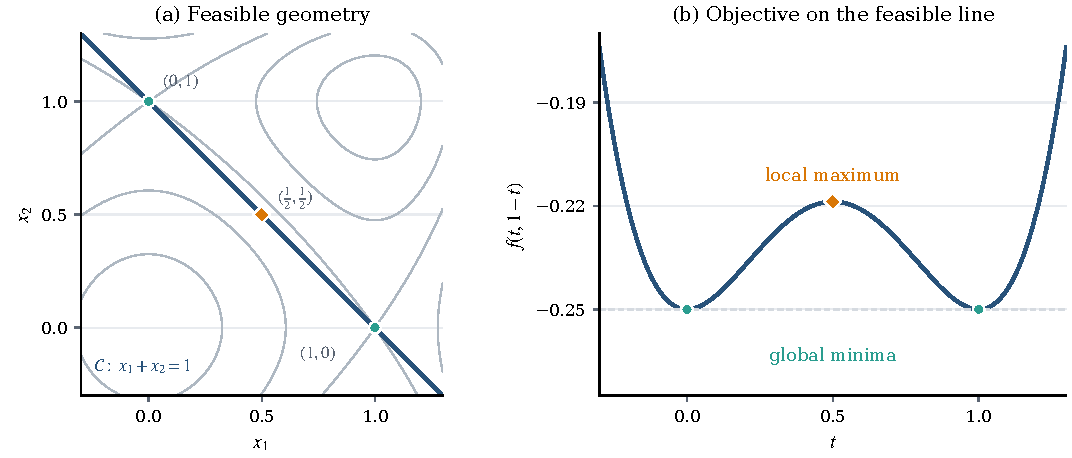
\includegraphics[width=\textwidth]{figures/affine_quartic_geometry.pdf}
  \caption{Geometry of the affine quartic example.  (a) Objective contours
  and the feasible line.  (b) The restriction to that line has two global
  minima and a central local maximum; their Lagrangian support thresholds
  are \(1\), \(1\), and \(3/4\), respectively.}
  \label{fig:affine-quartic-geometry}
\end{figure}

\subsubsection{False zeros from local inner minimization}

Below the safe threshold, the proximal model may be nonconvex.  It is then
incorrect to substitute an arbitrary local minimizer for the global infimum
in \cref{eq:sdg-decomposition}.  At the higher-valued local minimum of
\cref{eq:tilted-quartic}, denote the stationary point by
\(x_{\mathrm{hi}}\), the largest root of \(x^3-x+0.1=0\), with
\(x_{\mathrm{hi}}\approx0.9456492739\).  The center \(d=0\) remains a strict local
minimizer of the proximal model for every \(\beta\ge0\), since the coefficient
of \(d^2\) in \cref{eq:tilted-quartic-factorization} is positive there.
Nevertheless, when
\(\beta<1-x_{\mathrm{hi}}^2=\beta_{\crit}(x_{\mathrm{hi}},0)\), the same
factorization is negative near \(d=-2x_{\mathrm{hi}}\), so the center is not
globally minimizing.

The nonzero stationary displacements of the proximal model are available
explicitly:
\begin{equation}
  d_{\pm}(\beta)
  =
  \frac{-3x_{\mathrm{hi}}
  \pm\sqrt{\,4-3x_{\mathrm{hi}}^2-4\beta\,}}{2}.
  \label{eq:tilted-inner-stationary-branches}
\end{equation}
The branch \(d_-(\beta)\) gives the lower well throughout the tested range.
A center-initialized local solve instead remains at \(d=0\) for
\(\beta_x=0.05,0.08,0.10\) and therefore reports computed gap zero.
Evaluation of the explicit global branch gives respectively
\[
  0.10272358,\qquad 0.04670322,\qquad 0.01031227.
\]
The value-defined SDG remains positive at these parameters, whereas the
local-inner approximation returns a false zero.  The discrepancy is a
branch-selection error even though the quartic model is coercive and its
global minimum is attained.
\Cref{fig:threshold-diagnostics} juxtaposes the pair-dependent exact
thresholds in panel~(a) with this inner-solver failure in panel~(b).

\begin{figure}[htbp]
  \centering
  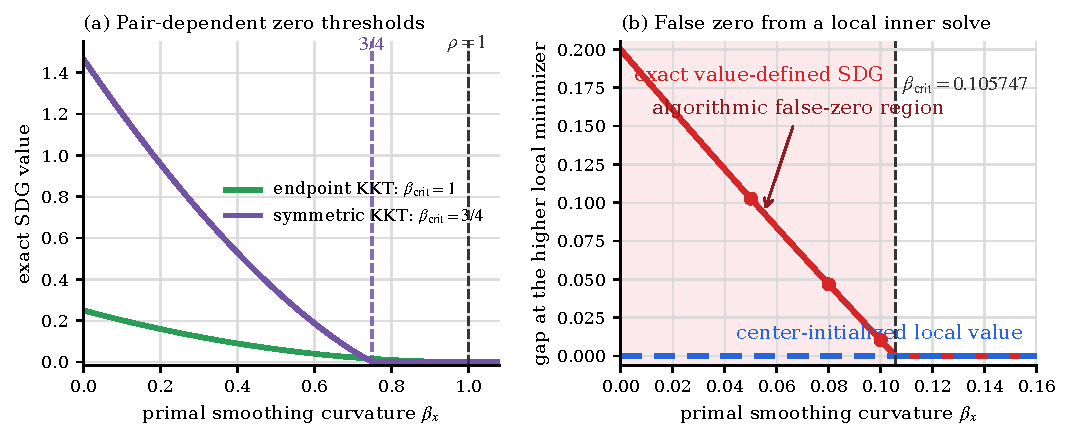
\includegraphics[width=\textwidth]{figures/threshold_diagnostics.pdf}
  \caption{Pointwise SDG thresholds and failure of a local inner
  solve.  (a) The exact gaps at the endpoint and symmetric KKT pairs vanish
  at \(\beta_x=1\) and \(3/4\), respectively.  (b) At the higher-valued local
  minimizer of the tilted quartic, the value-defined gap is positive for
  \(\beta_x<\beta_{\crit}\), whereas the center-initialized local branch
  returns zero.}
  \label{fig:threshold-diagnostics}
\end{figure}

These examples leave a different question after KKT detection: can a
stationary candidate be rejected using a feasible point of lower objective
value?  Reducing \(\beta_x\) does not answer this question.  A positive gap
then detects failure of a global quadratic support for the all-space
Lagrangian, which can occur even at a constrained global minimizer.
Moreover, evaluating that gap below the safe regime may require a nonconvex
global inner solve.

Instead, we keep proximal subproblems in the strongly convex regime and
change what they compare.  In \cref{sec:escape}, the candidate \(x\) is held
fixed, the center is perturbed along the feasible set, and the distinct map
\(P_\lambda^{\Cset}\) imposes the affine constraint inside each proximal
subproblem.  Its output can therefore be compared directly with \(f(x)\).
The resulting escape radius measures the perturbation needed to obtain
feasible descent, rather than the curvature needed to preserve a
Lagrangian support.
